\documentclass{beamer}

% Use the UiB theme
\usetheme{UiB}
% For strikethrough text using \sout
\usepackage[normalem]{ulem}

% For figures
\usepackage{graphicx}
\usepackage{tikz}
\usetikzlibrary{shapes.geometric,positioning,shapes.symbols,overlay-beamer-styles}

% Syntax Highlighting in code snippet
\usepackage{minted}

% Presentation metadata
\title{Everyone Is Better at Coding Than Me}
\subtitle{Developing A Modular IDE for Magnolia}
\author{Nils Michael Fitjar}
\institute{University of Bergen}
\date{\today}

\begin{document}
\section{Introduction}

\begin{frame}
    \frametitle{Topics}
    \begin{itemize}
      \item What an IDE is
      \item Why a create a new IDE
      \item Features
      \item Modularization
      \item Techstack
      \item Module Families and Granularity
      \item Conclusion
    \end{itemize}
\end{frame}

\section{What Is An IDE?}
\SectionPage

\begin{frame}
  \frametitle{The Solution To The Problem}
  \begin{quote}
    "It works on my machine." \textemdash Intern
  \end{quote}
  \begin{itemize}
    % TODO: Insert The Good, The Bad, and The Ugly picture, maybe?
    \item The Terminal, The Text Editor and The Compiler
  \end{itemize}
\end{frame}

\begin{frame}
  \frametitle{The Solution To The Problem}
  \begin{quote}
    "It works on my machine." \textemdash Intern
  \end{quote}
  \begin{itemize}
    % TODO: Insert The Good, The Bad, and The Ugly picture, maybe?
    \item The Terminal, The Text Editor and The Compiler
    \item Missing/incomplete:
    \begin{itemize}
      \item Libraries
      \item Environment variables
      \item Configurations
      \item Scripts
    \end{itemize}
  \end{itemize}
\end{frame}

\begin{frame}
  \frametitle{Integrated Development Environment}
  \begin{itemize}
    \item Bundle everything into a single application
    \item Easier to onboard new developers
    \item Other quality of life improvements
    \begin{itemize}
      \item File explorer
      \item Project manager
      \item Version Control System integration
      \item Syntax Highlighting
      \item Integrated debugging
      \item \dots
    \end{itemize}
  \end{itemize}
\end{frame}

\section{What? Why? What?}
\SectionPage

\begin{frame}
  \frametitle{Magnolia}
  \begin{itemize}
    \item A research programming language being developed by
      Bergen Language Design Laboratory at the University of Bergen
    \item Uses something called \textit{concepts}
    \item Similar to an Java interface.
    \item A concept declares
    \begin{itemize}
      \item Types
      \item Operations on those Types
      \item Axioms that specify the behavior of the Operations
    \end{itemize}
    \item A concept can use other concepts, and rename the Types and Operations
      in the concept, this is called renaming
    % TODO: Source?
    \item It is useful for a Magnolia Developer to be able to see the different
      renamings of a concept
  \end{itemize}
\end{frame}

\begin{frame}
    \frametitle{Simple Semigroup example}
    TODO: Add this
\end{frame}

\begin{frame}
    \frametitle{If It Ain't Broke}
    % TODO: Could probably expand this
    The current Magnolia IDE
    \begin{itemize}
        \item It uses an old version of Eclipse
        \item Uses deprecrated plugins
        \item Installation process is complex
        \item In INF220, two weeks is used to install it
    \end{itemize}
\end{frame}

\begin{frame}
  \frametitle{Forking VSCode And Adding AI}
  \begin{itemize}
    \item Current IDEs cannot have good support for experimental programming
      languages
    \item VSCode or similar IDEs could deprecrate needed functionality
    \item The installation process would then be complex
    \item Deep understanding of the used IDE is needed
  \end{itemize}
\end{frame}

\begin{frame}
  \frametitle{Why Modular?}
  \begin{itemize}
    \item Magnolia is still in development
    \item The Magnolia toolchain is being developed in parallel
    \item Nothing to create an integrated development environment with, yet.
    \item Modularity allows for future discoveries to be quickly adopted into
      the IDE
    \item Lowers the onboarding time for future maintainers
    % TODO: Add more
  \end{itemize}
\end{frame}

\section{Gimme, Gimme, Gimme}
\SectionPage

\begin{frame}
  \frametitle{(Features After Midnight)}
  \begin{itemize}
    \item Easy to extend with modules
      \begin{itemize}
        \item Low bar to create a module
        \item Easy to reason about how modules work together
      \end{itemize}
    \item Prototype modules should include these features:
      \begin{itemize}
        \item Can open, edit, delete files
        \item Has LSP support
        \item Can execute a program
      \end{itemize}
  \end{itemize}
\end{frame}

\begin{frame}
  \frametitle{Goals}
  % TODO: Should probably make these points more concrete
  \begin{itemize}
    \item Should be better than the current IDE
      \begin{itemize}
        \item Easy installation
        \item \textit{Lasts long} % TODO: Mention why this is good
      \end{itemize}
    \item Easy for the next \sout{sucker} developer to change core functionality
    \item Have a good plugin developer experience
  \end{itemize}
\end{frame}

\section{Creating The Everything App}
\SectionPage

\begin{frame}
  \frametitle{My hat is cooler than yours}
  \begin{quote}
    "When designing and developing an application, keep in mind your
    userbase" \textemdash Me, Just Now.
  \end{quote}
  \begin{itemize}
    \item The Developer, the main userbase
    \begin{itemize}
      \item Need plugins to have \textit{any} experience
    \end{itemize}
    \item The Module Developer, the secondary userbase
      \begin{itemize}
        \item Language Agnostic Module Architecture
        \item Good documentation and examples
        \item Should prioritize the Module Developer Experience
      \end{itemize}
    \item Maintainer Experience
      \begin{itemize}
        \item Good documentation
        \item Good testing
        % TODO: Unsure if I should mention this, as my CI/CD does not work, and
        % I am not sure if I am going to fix it
        \item CI\/CD
      \end{itemize}
  \end{itemize}
\end{frame}

\begin{frame}
  \frametitle{What Is A Module?}
  \begin{itemize}
    \item Third Party Code to be executed/interpereted
      \begin{itemize}
        \item Tailormade Scripting Language
        \item An already existing programming language
      \end{itemize}
  \end{itemize}
\end{frame}

\begin{frame}
  \frametitle{How To Model A Module?}
  \begin{itemize}
    \item A module needs to:
      \begin{itemize}
        \item Initialize some state
        \item Update the state based on events
        \item Render the view based on the state
      \end{itemize}
    \item Module architecture is inspired by Elm and MVC
    \item A Module exposes three functions:
      \begin{itemize}
        \item Init \textemdash to set the state
        \item Update \textemdash to update the state based on Messages (Msg)
        \item View \textemdash to render the view based on the state
      \end{itemize}
    \item Like Elm, events like, \textit{onClick}, are sent as Msg
    \item init \to update \to view \to update \to \dots cycle
    \item A module should be \textit{pure}
  \end{itemize}
\end{frame}

\begin{frame}
  \frametitle{Module Architecture}
  \centering
  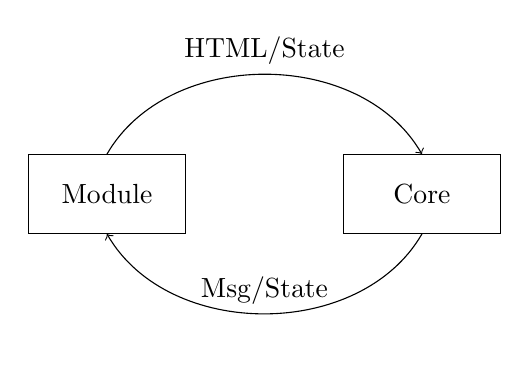
\begin{tikzpicture}
    % Nodes
    \node (p) [rectangle, draw, minimum height=1cm, minimum width=2cm] at (0, 0) {Module};
    \node (i) [rectangle, draw, minimum height=1cm, minimum width=2cm] at (4, 0) {Core};
    % Arrow
    \draw[->] (p.north) to[out=60, in=120] node[midway, above] {HTML/State} (i.north);
    \draw[->] (i.south) to[out=-120, in=-60] node[midway, above] {Msg/State} (p.south);
    % Header
  \end{tikzpicture}
\end{frame}

\begin{frame}
  \frametitle{Haskell "Counter"-Example}
  \begin{minted}{Haskell}
    init :: State
    init = [("counter", Int 0)]

    update :: Msg -> State -> State
    update (Msg "counter" (Int i)) state =
    case lookup "counter" state of
    Just (Int j) -> [("counter", Int (j + i))]
    Nothing -> [("counter", Int 0)]
    update _ _ = []

    view :: State -> HTML
    view state = Div [class "container"]
    [ Text "Hello, World!"
    , Btn [OnClick $ Msg "counter" (Int 1)] []
    , Text $ putStrLn $ lookup "counter" state
    ]
  \end{minted}
\end{frame}


\begin{frame}
  \frametitle{Tech \sout{Heap} Stack}
  \begin{itemize}
    \item Rust, because it is a low level system language
  \end{itemize}
\end{frame}

\begin{frame}
  \frametitle{Tech \sout{Heap} Stack}
  \begin{itemize}
    \item Rust, because it is a low level system language
      \begin{itemize}
        \item Compiler knows when a value is unused
      \end{itemize}
  \end{itemize}
\end{frame}

\begin{frame}
  \frametitle{Tech \sout{Heap} Stack}
  \begin{itemize}
    \item Rust, because it is a low level system language
      \begin{itemize}
        \item Compiler knows when a value is unused
        \item Automatically \textit{dropped}
      \end{itemize}
  \end{itemize}
\end{frame}

\begin{frame}
  \frametitle{Tech \sout{Heap} Stack}
  \begin{itemize}
    \item Rust, because it is a low level system language
      \begin{itemize}
        \item Compiler knows when a value is unused
        \item Automatically \textit{dropped}
        \item No dangling pointers/null references or memory leakage*
      \end{itemize}
  \end{itemize}
\end{frame}

\begin{frame}
  \frametitle{Tech \sout{Heap} Stack}
  \begin{itemize}
    \item Rust, because it is a low level system language
      \begin{itemize}
        \item Compiler knows when a value is unused
        \item Automatically \textit{dropped}
        \item No dangling pointers/null references
      \end{itemize}
    \item Tauri, UI components can be created using JavaScript
  \end{itemize}
\end{frame}

\begin{frame}
  \frametitle{Tech \sout{Heap} Stack}
  \begin{itemize}
    \item Rust, because it is a low level system language
      \begin{itemize}
        \item Compiler knows when a value is unused
        \item Automatically \textit{dropped}
        \item No dangling pointers/null references
      \end{itemize}
    \item Tauri, UI components can be created using JavaScript
    \item Splits the core application into two parts, loosely coupled parts
  \end{itemize}
\end{frame}

\begin{frame}
  \frametitle{Tech \sout{Heap} Stack}
  \begin{itemize}
    \item Rust, because it is a low level system language
      \begin{itemize}
        \item Compiler knows when a value is unused
        \item Automatically \textit{dropped}
        \item No dangling pointers/null references
      \end{itemize}
    \item Tauri, UI components can be created using JavaScript
    \item Splits the core application into two parts, loosely coupled parts
      \begin{itemize}
        \item Frontend (JavaScript)
        \item Backend (Rust)
      \end{itemize}
  \end{itemize}
\end{frame}

\begin{frame}
  \frametitle{Tech \sout{Heap} Stack}
  \begin{itemize}
    \item Rust, because it is a low level system language
      \begin{itemize}
        \item Compiler knows when a value is unused
        \item Automatically \textit{dropped}
        \item No dangling pointers/null references
      \end{itemize}
    \item Tauri, UI components can be created using JavaScript
    \item Splits the core application into two parts, loosely coupled parts
      \begin{itemize}
        \item Frontend (JavaScript)
        \item Backend (Rust)
      \end{itemize}
    \item Communication is like JSON-RPC, which, effectively, is the same as a
      client-server
  \end{itemize}
\end{frame}

\begin{frame}
  \frametitle{Tech \sout{Heap} Stack}
  \begin{itemize}
    \item Rust, because it is a low level system language
      \begin{itemize}
        \item Compiler knows when a value is unused
        \item Automatically \textit{dropped}
        \item No dangling pointers/null references
      \end{itemize}
    \item Tauri, UI components can be created using JavaScript
    \item Splits the core application into two parts, loosely coupled parts
      \begin{itemize}
        \item Frontend (JavaScript)
        \item Backend (Rust)
      \end{itemize}
    \item Communication is like JSON-RPC, which, effectively, is the same as a
      client-server
    \item Allows for modules in two different languages, with little effort.
      I hoped.
  \end{itemize}
\end{frame}


\section{The Frontend}
\SectionPage

\begin{frame}
  \frametitle{I Need Super Computer Time For My Featureless App}
  \begin{itemize}
    \item JavaScript is more \textit{unsafe} than Rust, due of a lack of typing
      and restrictions
  \end{itemize}
\end{frame}

\begin{frame}
  \frametitle{I Need Super Computer Time For My Featureless App}
  \begin{itemize}
    \item JavaScript is more \textit{unsafe} than Rust, due of a lack of typing
      and restrictions
    \item Need to decode the output from the modules, and catch any exceptions
  \end{itemize}
\end{frame}

\begin{frame}
  \frametitle{I Need Super Computer Time For My Featureless App}
  \begin{itemize}
    \item JavaScript is more \textit{unsafe} than Rust, due of a lack of typing
    \item Need to decode the output from the modules, and catch any exceptions
    \item When implementing the init \to update \to view - cycle, I tested with
      a \textit{basic} module, which should only display "Hello, World!"
  \end{itemize}
\end{frame}

\begin{frame}
  \frametitle{I Need Super Computer Time For My Featureless App}
  \begin{itemize}
    \item JavaScript is more \textit{unsafe} than Rust, due of a lack of typing
    \item Need to decode the output from the modules, and catch any exceptions
    \item When implementing the init \to update \to view - cycle, I tested with
      a \textit{basic} module, which should only display "Hello, World!"
      \begin{itemize}
        \item The module initialized the state
      \end{itemize}
  \end{itemize}
\end{frame}

\begin{frame}
  \frametitle{I Need Super Computer Time For My Featureless App}
  \begin{itemize}
    \item JavaScript is more \textit{unsafe} than Rust, due of a lack of typing
    \item Need to decode the output from the modules, and catch any exceptions
    \item When implementing the init \to update \to view - cycle, I tested with
      a \textit{basic} module, which should only display "Hello, World!"
      \begin{itemize}
        \item The module initialized the state
        \item It rendered the view
      \end{itemize}
  \end{itemize}
\end{frame}

\begin{frame}
  \frametitle{I Need Super Computer Time For My Featureless App}
  \begin{itemize}
    \item JavaScript is more \textit{unsafe} than Rust, due of a lack of typing
    \item Need to decode the output from the modules, and catch any exceptions
    \item When implementing the init \to update \to view - cycle, I tested with
      a \textit{basic} module, which should only display "Hello, World!"
      \begin{itemize}
        \item The module initialized the state
        \item It rendered the view
        \item Somehow triggered an update
      \end{itemize}
  \end{itemize}
\end{frame}

\begin{frame}
  \frametitle{I Need Super Computer Time For My Featureless App}
  \begin{itemize}
    \item JavaScript is more \textit{unsafe} than Rust, due of a lack of typing
    \item Need to decode the output from the modules, and catch any exceptions
    \item When implementing the init \to update \to view - cycle, I tested with
      a \textit{basic} module, which should only display "Hello, World!"
      \begin{itemize}
        \item The module initialized the state
        \item It rendered the view
        \item Somehow triggered an update
        \item Which triggered a rerender
      \end{itemize}
  \end{itemize}
\end{frame}

\begin{frame}
  \frametitle{I Need Super Computer Time For My Featureless App}
  \begin{itemize}
    \item JavaScript is more \textit{unsafe} than Rust, due of a lack of typing
    \item Need to decode the output from the modules, and catch any exceptions
    \item When implementing the init \to update \to view - cycle, I tested with
      a \textit{basic} module, which should only display "Hello, World!"
      \begin{itemize}
        \item The module initialized the state
        \item It rendered the view
        \item Somehow triggered an update
        \item Which triggered a rerender
        \item Which triggered an update
      \end{itemize}
  \end{itemize}
\end{frame}

\begin{frame}
  \frametitle{I Need Super Computer Time For My Featureless App}
  \begin{itemize}
    \item JavaScript is more \textit{unsafe} than Rust, due of a lack of typing
    \item Need to decode the output from the modules, and catch any exceptions
    \item When implementing the init \to update \to view - cycle, I tested with
      a \textit{basic} module, which should only display "Hello, World!"
      \begin{itemize}
        \item The module initialized the state
        \item It rendered the view
        \item Somehow triggered an update
        \item Which triggered a rerender
        \item Which triggered an update
        \item Which triggered a rerender
      \end{itemize}
  \end{itemize}
\end{frame}

\begin{frame}
  \frametitle{I Need Super Computer Time For My Featureless App}
  \begin{itemize}
    \item JavaScript is more \textit{unsafe} than Rust, due of a lack of typing
    \item Need to decode the output from the modules, and catch any exceptions
    \item When implementing the init \to update \to view - cycle, I tested with
      a \textit{basic} module, which should only display "Hello, World!"
      \begin{itemize}
        \item The module initialized the state
        \item It rendered the view
        \item Somehow triggered an update
        \item Which triggered a rerender
        \item Which triggered an update
        \item Which triggered a rerender
        \item \dots
      \end{itemize}
  \end{itemize}
\end{frame}

\begin{frame}
  \frametitle{I Need Super Computer Time For My Featureless App}
  \begin{figure}
    \centering
    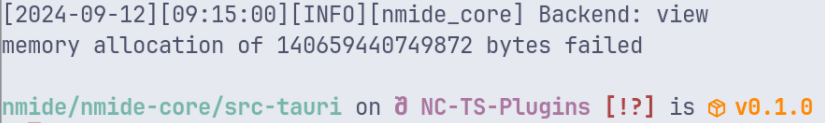
\includegraphics[width=0.8\textwidth]{./pics/memory-allocation-zoomed.png}
    %\caption{Stress Testing}
  \end{figure}
  It's just 140.6594 TeraBytes, which is a meager 15 \% of the total memory of NASA's
  supercomputer
\end{frame}

\begin{frame}
  \frametitle{But Can It Run Doom?}
  \begin{itemize}
    \item JavaScript plugin allows for reusing existing JavaScript libraries
  \end{itemize}
\end{frame}

\begin{frame}
  \frametitle{But Can It Run Doom?}
  \begin{itemize}
    \item JavaScript plugin allows for reusing existing JavaScript libraries
    \item So, you can play Doom
  \end{itemize}
\end{frame}

\begin{frame}
  \begin{center}
    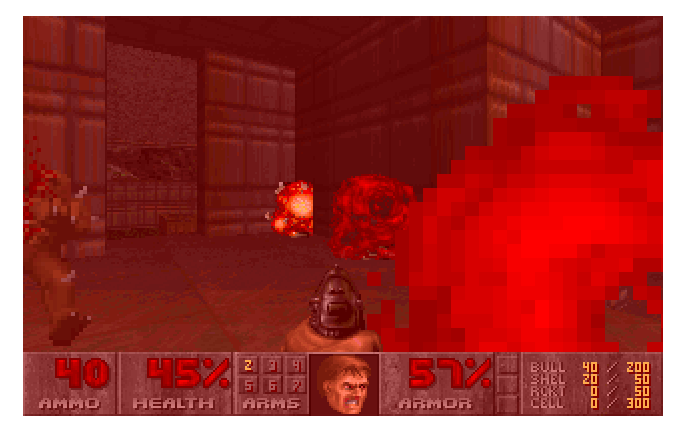
\includegraphics[width=0.95\textwidth]{./pics/doom.png}
    %\caption{Doom using js-dos}
  \end{center}
\end{frame}


\section{The Backend}
\SectionPage

\begin{frame}
  \frametitle{Blasingly Fast Memory Leakage}
  \begin{itemize}
    \item The Rust ABI is not protected by their semver notation
  \end{itemize}
\end{frame}

\begin{frame}
  \frametitle{Blasingly Fast Memory Leakage}
  \begin{itemize}
    \item The Rust ABI is not protected by their semver notation
    \item This means that even a patch to the Rust compiler can break a
      Rust Module
  \end{itemize}
\end{frame}

\begin{frame}
  \frametitle{Blasingly Fast Memory Leakage}
  \begin{itemize}
    \item The Rust ABI is not protected by their semver notation
    \item This means that even a patch to the Rust compiler can break a
      Rust Module
    \item Can be fixed by using a Rust Library: \textit{abi\_stable}
  \end{itemize}
\end{frame}

\begin{frame}
  \frametitle{Blasingly Fast Memory Leakage}
  \begin{itemize}
    \item The Rust ABI is not protected by their semver notation
    \item This means that even a patch to the Rust compiler can break a
      Rust Module
    \item Can be fixed by using a Rust Library: \textit{abi\_stable}
    \item Had to use `ManuallyDrop` for more complex types, which disables
      the automatic drop
  \end{itemize}
\end{frame}

\begin{frame}
  \frametitle{Blasingly Fast Memory Leakage}
  \begin{itemize}
    \item The Rust ABI is not protected by their semver notation
    \item This means that even a patch to the Rust compiler can break a
      Rust Module
    \item Can be fixed by using a Rust Library: \textit{abi\_stable}
    \item Had to use `ManuallyDrop` for more complex types, which disables
      the automatic drop
    \item Fixed by having Rust modules only reference the state, meaning
      after update and view, the module can be safely dropped
  \end{itemize}
\end{frame}

\hidelogo
\begin{frame}
  \frametitle{Core Flowdiagram}
  \centering
  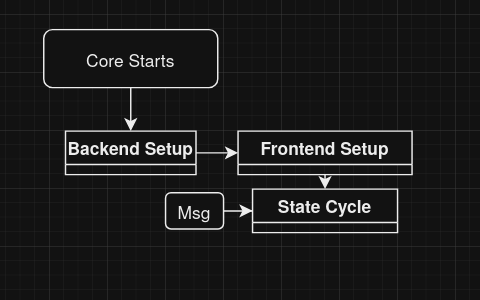
\includegraphics[width=0.95\textwidth]{./pics/mini-core-cycle.png}
  %\caption{Flowdiagram of the Cores start up sequence}
\end{frame}

\begin{frame}
  \frametitle{Backend Setup}
  \centering
  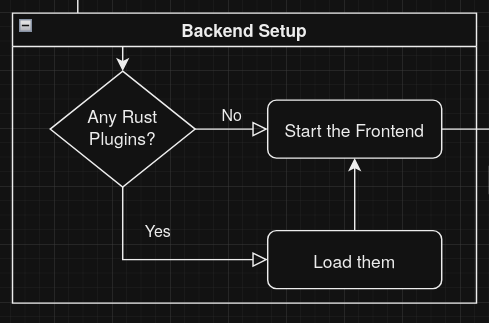
\includegraphics[width=0.95\textwidth]{./pics/backend-setup.png}
  %\caption{Flowdiagram of the Backend start up sequence}
\end{frame}

\begin{frame}
  \frametitle{Frontend Setup}
  \centering
  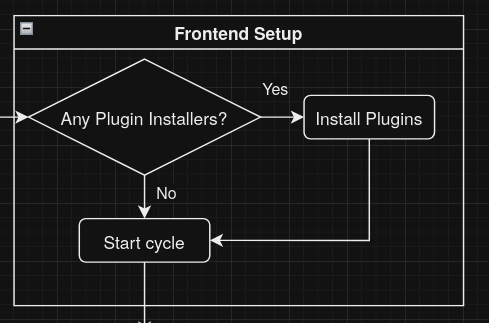
\includegraphics[width=0.95\textwidth]{./pics/frontend-setup.png}
  %\caption{Flowdiagram of the Frontend start up sequence}
\end{frame}

\begin{frame}
  \frametitle{State Cycle}
  \centering
  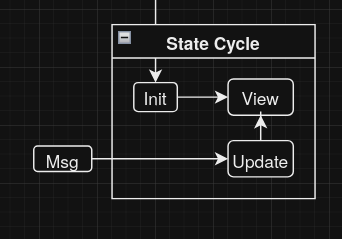
\includegraphics[width=0.9\textwidth]{./pics/state-cycle.png}
  %\caption{Flowdiagram of the state cycle}
\end{frame}

\section{Modularity and Granularity}
\SectionPage

\showlogo
\begin{frame}
  \frametitle{How To Get Features}
  \begin{itemize}
    \item Can make one IDE module
    \item But granularity is more fun
    \item Prototype Modules
      \begin{itemize}
        \item Module Debugger
          \begin{itemize}
            \item Display State
            \item Display Msgs being sent
            \item Toggable Modules
          \end{itemize}
        \item Dependency Viewer
          \begin{itemize}
            \item Showcase integration with existing JavaScript libraries
          \end{itemize}
        \item Rendering Framework
      \end{itemize}
    \item IDE Family
      \begin{itemize}
        \item File System
        \item File Explorer
        \item Text Editor
        \item Rendering Framework
      \end{itemize}
  \end{itemize}
\end{frame}

\begin{frame}
  \frametitle{Pureness or Modularity}
  \begin{itemize}
    \item When implementing the prototype modules
      \begin{itemize}
        \item JavaScript is more useful when directly manipulating the DOM
        \item Creating HTML-trees in Rust is cumbersome, but doing file
          operations is trivial
      \end{itemize}
    \item Design the core to allow for impureness, by exposing core
      functionality
      \begin{itemize}
        \item Module locations
        \item Module installation
        \item Client used for Backend communication
        \item Error logging
        \item Where HTML is placed
        \item How HTML is cleaned up
        \item Access to installed plugins
      \end{itemize}
    \item The Core can be \textit{trivially} turned into a web-based application
  \end{itemize}
\end{frame}

\begin{frame}
  \frametitle{IDE Family Diagram}
    \centering
    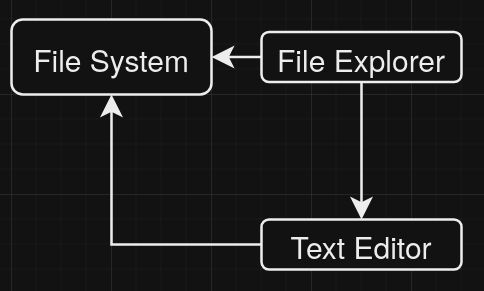
\includegraphics[width=0.9\textwidth]{./pics/ide-family.png}
\end{frame}

% Another section
\section{Conclusion}
\SectionPage

\begin{frame}
  \frametitle{Making An IDE Is Hard}
  \begin{figure}
    \centering
    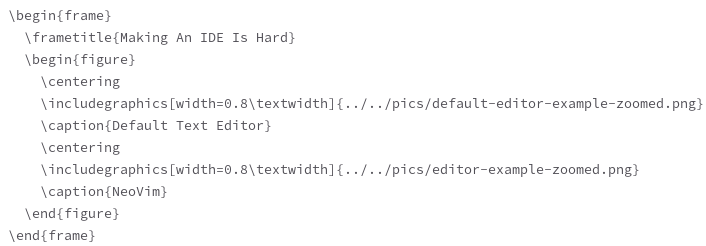
\includegraphics[width=0.8\textwidth]{./pics/default-editor-example-zoomed.png}
    %\caption{Default Text Editor}
    \centering
    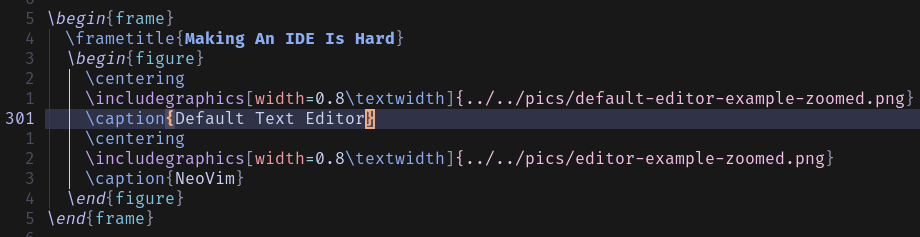
\includegraphics[width=0.8\textwidth]{./pics/editor-example-zoomed.png}
    %\caption{NeoVim}
  \end{figure}
\end{frame}

\begin{frame}
    \frametitle{Making An IDE Is Hard}
    \begin{figure}
      \centering
      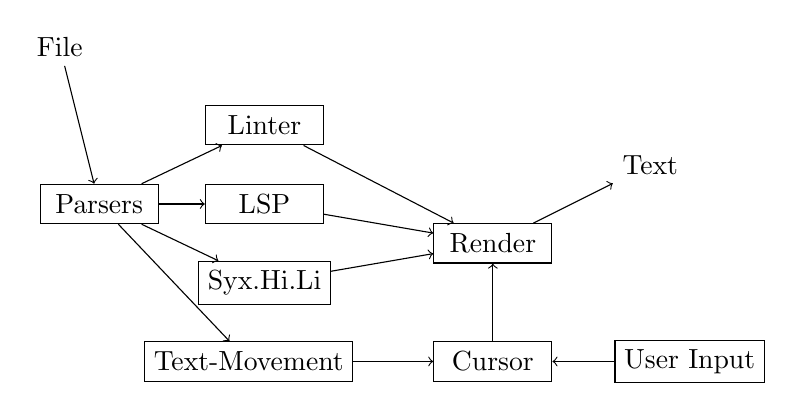
\begin{tikzpicture}
        % Nodes
        \node (file) [] at (-6, 3) {File};
        \node (parser) [rectangle, draw, minimum height=0.5cm, minimum width=1.5cm] at (-5.5, 1) {Parsers};
        \node (lsp) [rectangle, draw, minimum height=0.5cm, minimum width=1.5cm] at (-3.4, 1) {LSP};
        \node (stxhili) [rectangle, draw, minimum height=0.5cm, minimum width=1.5cm] at (-3.4, 0) {Syx.Hi.Li};
        \node (text-movement) [rectangle, draw, minimum height=0.5cm, minimum width=1.5cm] at (-3.6, -1) {Text-Movement};
        \node (linter) [rectangle, draw, minimum height=0.5cm, minimum width=1.5cm] at (-3.4, 2) {Linter};
        \node (cursor) [rectangle, draw, minimum height=0.5cm, minimum width=1.5cm] at (-0.5, -1) {Cursor};
        \node (user-input) [rectangle, draw, minimum height=0.5cm, minimum width=1.5cm] at (2, -1) {User Input};
        \node (render) [rectangle, draw, minimum height=0.5cm, minimum width=1.5cm] at (-0.5, 0.5) {Render};
        \node (text) at (1.5, 1.5) {Text};
        % Arrow
        \draw[->] (file) -- (parser) node[midway, above] {};
        \draw[->] (parser) -- (lsp) node[midway, above] {};
        \draw[->] (parser) -- (stxhili) node[midway, above] {};
        \draw[->] (parser) -- (linter) node[midway, above] {};
        \draw[->] (parser) -- (text-movement) node[midway, above] {};
        \draw[<-] (render) -- (lsp) node[midway, above] {};
        \draw[<-] (render) -- (stxhili) node[midway, above] {};
        \draw[<-] (render) -- (linter) node[midway, above] {};
        \draw[<-] (cursor) -- (text-movement) node[midway, above] {};
        \draw[<-] (cursor) -- (user-input) node[midway, above] {};
        \draw[->] (cursor) -- (render) node[midway, above] {};
        \draw[->] (render) -- (text) node[midway, above] {};
      \end{tikzpicture}
      %\caption{Granular Editor}
    \end{figure}
\end{frame}

\end{document}
